% tikzposter.tex, version 2.0
% Original template created by Elena Botoeva [botoeva@inf.unibz.it], June 2012
% 
% This file is distributed under the Creative Commons Attribution-NonCommercial 2.0
% Generic (CC BY-NC 2.0) license
% http://creativecommons.org/licenses/by-nc/2.0/ 


\documentclass{a0poster}

\usepackage{fancytikzposter} 


%%%%% --------- Change here if you want ---------- %%%%%
%% margin for the geometry package, must be changed before using the geometry package
%% default value is 4cm
% \setmargin{4}

%% the space between the blocks
%% default value is 2cm
% \setblockspacing{2}

%% the height of the title stripe in block nodes, decrease it to save space
%% default value is 3cm
% \setblocktitleheight{3}

%% the number of columns in the poster, possible values 2,3
%% default value is 2
% \setcolumnnumber{3}

%% the space between two or more groups of authors from different institutions
%% used in \maketitle
% \setinstituteshift{10}

%% which template to use
%% N1 simple, standard look, with a colored background and gray boxes
%% N2 board with nodes
%% N3 another standard look
%% N4 envelope-like look
%% N5 with a wave-like head, original idea taken from
%%%% http://fc09.deviantart.net/fs71/f/2010/322/1/1/scientific_poster_by_nabuy-d333ria.jpg
\usetemplate{3}

%% components of the templates
%% (the maximal possible numbers are mentioned as the parameters)
%\usecolortemplate{3}
% \usebackgroundtemplate{1}
% \usetitletemplate{2}
% \useblocknodetemplate{5}
% \useplainnodetemplate{4}
% \useinnernodetemplate{2}


%% the height of the head drawing on top 
%% applicable to templates N3, 4 and 5
% \setheaddrawingheight{14}


%% change the basic colors
\definecolor{myblue}{HTML}{008888} 
\setfirstcolor{orange}% default 116699
\setsecondcolor{white}% default CCCCCC
%\setsecondcolor{gray!80!}% default CCCCCC
%\setthirdcolor{orange!100!yellow}% default 991111
\setthirdcolor{orange}% default 991111


%% change the more specific colors
% \setbackgrounddarkcolor{colorone!70!black}
% \setbackgroundlightcolor{colorone!70!black}
% \settitletextcolor{textcolor}
% \settitlefillcolor{white}
% \settitledrawcolor{colortwo}
% \setblocktextcolor{textcolor}
% \setblockfillcolor{white}
 \setblocktitletextcolor{white}
 \setblocktitlefillcolor{colorthree} %the color of the border
% \setplainblocktextcolor{textcolor}
% \setplainblockfillcolor{colorthree!40!}
% \setplainblocktitletextcolor{textcolor}
% \setplainblocktitlefillcolor{colorthree!60!}
% \setinnerblocktextcolor{textcolor}
%\setinnerblockfillcolor{white}
% \setinnerblocktitletextcolor{white}
% \setinnerblocktitlefillcolor{colorthree}




%%% size of the document and the margins
%% A0
% \usepackage[margin=\margin cm, paperwidth=118.9cm, paperheight=84.1cm]{geometry} 
\usepackage[margin=\margin cm, paperwidth=84.1cm, paperheight=118.9cm]{geometry}
%% B1
% \usepackage[margin=\margin cm, paperwidth=70cm, paperheight=100cm]{geometry}



%% changing the fonts
\usepackage{cmbright}
%\usepackage[default]{cantarell}
%\usepackage{avant}
%\usepackage[math]{iwona}
%\usepackage[amsmath]
\usepackage[T1]{fontenc}


%% add your packages here
%\usepackage{graphics}
%\usepackage{graphicx}
%%\usepackage{wasysym}
%\usepackage{pgf}
%\usepackage{verbatim}
%\usepackage{tikz}
%\usepackage{pgfmath}
%\usetikzlibrary{calc}
%\usetikzlibrary{backgrounds}
%\usetikzlibrary{arrows}
%\usetikzlibrary{shapes.arrows}
%\usetikzlibrary{shapes.geometric}
%\usetikzlibrary{decorations.markings}
%\usetikzlibrary{positioning}
%\usetikzlibrary{fit,chains}

\newcommand{\beq}{\begin{equation}}
\newcommand{\eeq}{\end{equation}}
\newcommand{\beqa}{\begin{eqnarray}}
\newcommand{\eeqa}{\end{eqnarray}}
\newcommand{\bi}{\begin{itemize}}
\newcommand{\ei}{\end{itemize}}
\newcommand{\ket} [1] {\vert #1 \rangle}
\newcommand{\bra} [1] {\langle #1 \vert}
\newcommand{\braket}[2]{\langle #1 | #2 \rangle}
\newcommand{\ev}[1]{\langle #1 \rangle}
\newcommand{\vbra}[1]{\left ( #1 \right |}
\newcommand{\vket}[1]{\left |#1 \right )}
\newcommand{\vbraket}[2]{\left ( #1 \middle |#2 \right )} 
\newcommand{\braopket}[3]{\left \langle #1 \middle |#2 \middle | #3 \right \rangle} 
\newcommand{\vbraopket}[3]{\left ( #1 \middle |#2 \middle | #3 \right )} 

%\newcommand<>{\highlighton}[1]{%
%  \alt#2{\structure{#1}}{{#1}}
%}

\newcommand{\icon}[1]{\pgfimage[height=1em]{#1}}

\usepackage{empheq}

\newlength\mytemplen
\newsavebox\mytempbox

\makeatletter
\newcommand\mybluebox{%
    \@ifnextchar[%]
       {\@mybluebox}%
       {\@mybluebox[0pt]}}

\def\@mybluebox[#1]{%
    \@ifnextchar[%]
       {\@@mybluebox[#1]}%
       {\@@mybluebox[#1][0pt]}}

\def\@@mybluebox[#1][#2]#3{
    \sbox\mytempbox{#3}%
    \mytemplen\ht\mytempbox
    \advance\mytemplen #1\relax
    \ht\mytempbox\mytemplen
    \mytemplen\dp\mytempbox
    \advance\mytemplen #2\relax
    \dp\mytempbox\mytemplen
    \fcolorbox{airlightblue}{white}{\hspace{1em}\usebox{\mytempbox}\hspace{1em}}}

\makeatother

\tikzset{peps/.style={circle=2pt,draw=black!100,fill=green!50,inner sep=3pt}}
\tikzset{bpeps/.style={circle=2pt,draw=black!100,thick,fill=green!50,inner sep=3pt}}
\tikzset{gamma/.style={circle=2pt,draw=black!100,fill=blue!20,inner sep=3pt}}
\tikzset{lambda/.style={rectangle,rotate=45,draw=black!100,fill=orange!50,inner sep=4pt}}
\tikzset{operator/.style={circle=2pt,draw=black!100,fill=orange!80,inner sep=3pt}}
\tikzset{cdot/.style={circle=2pt,draw=black!100,fill=white,inner sep=1pt}}
\tikzset{bg/.style={rounded corners,thin,fill=blue!10}}
\tikzset{inv/.style={opacity=0}}
\tikzset{spin/.style={circle=2pt,draw=black!100,fill=orange!80,inner sep=3pt}}
\tikzset{unitbox/.style={fill=black!3,rounded corners}}
\tikzset{corner/.style={rectangle=10pt,fill=blue!50,draw=black}}
\tikzset{side/.style={rectangle=6pt,fill=blue!20,draw=black}}
\tikzset{cside/.style={circle=6pt,fill=blue!20,draw=black}}
\tikzset{swapg/.style={circle=1pt,draw=black,fill=black!80,inner sep=1pt}}

\tikzset{base/.style={circle=2pt,fill=orange!80,draw=black}}
\tikzset{det/.style={circle=2pt,fill=blue!20,draw=black,inner sep=4pt}}
\tikzset{iso/.style={circle=2pt,fill=red!20,draw=black,inner sep=4pt}}
\tikzset{top/.style={circle=2pt,fill=black!20,draw=black,inner sep=4pt}}
\tikzset{siso/.style={circle=1pt,fill=red!20,draw=black,inner sep=1pt}}

%Brayden's
\tikzset{GHZ/.style={circle=2pt,fill=black!80,draw=black,inner sep=2pt}}
\tikzset{X/.style={circle=2pt,fill=black!80,text=white,font=\footnotesize, draw=black,inner sep=1pt}}
\tikzset{W/.style={circle=2pt,fill=black!20,draw=black,double,inner sep=2pt}}
\tikzset{eli/.style={ellipse, rotate=0, draw=black, fill=gray!20}}

%http://tex.stackexchange.com/questions/199683/how-to-plot-quantum-logical-gates-with-tikz
\tikzset{
cross/.style={path picture={ 
            \draw[thick,black](path picture bounding box.north) -- (path picture bounding                  box.south) (path picture bounding box.west) -- (path picture bounding                      box.east);
            }},
crossx/.style={path picture={ 
            \draw[thick,black,inner sep=0pt]
                (path picture bounding box.south east) -- (path picture bounding box.north west) (path picture bounding box.south west) -- (path picture bounding box.north east);
            }},
circlewc/.style={circle=2pt,draw, crossx}
}


\title{Featureless Bosonic Insulators}
\author{Brayden Ware\\
  UCSB \And Itamar Kimchi\\ UCB  \And Siddarth Parameswaran \\ UCI  \And Bela Bauer \\ Station Q }


\begin{document}

%%%%% ---------- the background picture ---------- %%%%%
%% to change it modify the macro \BackgroundPicture
\ClearShipoutPicture
\AddToShipoutPicture{\BackgroundPicture}

\noindent % to have the picture right in the center
\begin{tikzpicture}
  \initializesizeandshifts
  % \setxshift{15}
  % \setyshift{2}


  %% the title block, #1 - shift, the default value is (0,0), #2 - width, #3 - scale
  %% the alias of the title block is `title', so we can refer to its boundaries later
  \titleblock{47}{1.5}

  %% a logo can be added to the title block
  %% #1 - anchor relative to the title block, #2 - shift, #3 - width, #3 - file name
  % \ifthenelse{\equal{\template}{2}}{ 
  %   \addlogo[south west]{(2,0)}{6cm}{unibz_b.png}
  % }{
  %   \addlogo[south west]{(2,0)}{6cm}{unibz_w.png}
  % }


  %% a block node, with the specified position (optional), title and the content
  %% #1 - where (optional), #2 - title, #3 - text
  %%%%%%%%%% ------------------------------------------ %%%%%%%%%%
 \blocknode
{Block with inner block}
{
\begin{center}
    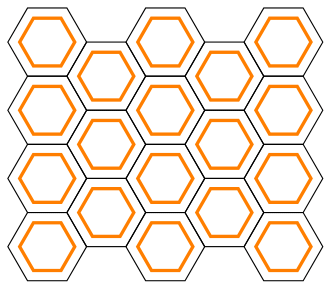
\includegraphics[width=6in]{diagrams/fbi3.png}
\end{center}
}  
  


  %% a callout node
  %% #1 - rotate angle (optional), #2 - from, #3 - where, #4 - width, #5 - text
  %%%%%%%%%% ------------------------------------------ %%%%%%%%%%
%  \calloutnode {($(box.center)+(-2,-8)$)}
%  {($(box.center)+(10,-1)$)}
%  {19cm}
%  {\small
%    Macro for creating a block node:
%    \begin{itemize}
%    \item[] \textbackslash blocknode\{Block Title\}\{Block Content\}
%    \end{itemize}
%    Macro \textbackslash blocknode has three parameters. The first one is
%    optional and it is the position of the block. The first block will be
%    automatically placed to (\$(firstrow)-(xshift)-(yshift)\$), which is the
%    left corner below the title block. In most of the templates, (firstrow) is
%    set to (title.south), where \emph{title} is the alias for the title
%    block. Each subsequent block is automatically placed to
%    [(\$(box.south)-(yshift)\$)], i.e., below the previous block aliased
%    \emph{box}.  You can also use an explicit parameter, e.g., $(-10,30)$ (note
%    that (0,0) is the center of the poster). The second parameter is the title
%    of the block. Finally, the last parameter is the  actual content. 
%  }




  %% by default, the position of the new block node is right below the previous
  %% block node, stored in (currenty)
  %% box is the alias of the previous block, so we can refer to its boundaries

  %%%%%%%%%% ------------------------------------------ %%%%%%%%%%
  \blocknode{Standard Text Block: How to put authors in}%
  {To make title, use the standard commands \textbackslash title and
    \textbackslash author in the preamble, and then the following macro:
    \begin{itemize}
    \item[] \textbackslash titleblock\{50\}\{1.5\}
    \end{itemize}
    Macro \textbackslash titleblock has three parameters. The first one is
    optional and it specifies the shift of the title block w.r.t.\ its default
    position, which is set to (\$0.5*(0,\textbackslash
    paperheight)-(0,\textbackslash margin)\$). The second parameter is the width
    of the title block, and the third parameter is the scaling ratio (to make
    the title bigger or smaller).\\

    \small
    The syntax for specifying authors is similar to the one in aaai.sty.  Author
    information can be set in various styles: For several authors from the same
    institution:
    \begin{itemize}\item[] 
      \textbackslash author\{Author 1 \textbackslash and ... \textbackslash and
      Author n \textbackslash\textbackslash\\ 
      Address line \textbackslash\textbackslash \
      ... \textbackslash\textbackslash \ Address line\}
    \end{itemize}

    If the names do not fit well on one line use
    \begin{itemize}\item[] 
      \textbackslash author\{Author 1 \textbackslash\textbackslash \
      \{\textbackslash bf Author 2\} \textbackslash\textbackslash \
      ... \textbackslash\textbackslash \
      \{\textbackslash bf Author n\} \textbackslash\textbackslash\\
      Address line \textbackslash\textbackslash \
      ... \textbackslash\textbackslash \ Address line\}
    \end{itemize}

    For authors from different institutions: 
    \begin{itemize}\item[] 
      \textbackslash author\{Author 1 \textbackslash\textbackslash \ Address
      line \textbackslash\textbackslash \ ... \textbackslash\textbackslash \
      Address line \\ \textbackslash And ... \textbackslash And \\
      Author n \textbackslash\textbackslash \ Address line
      \textbackslash\textbackslash \ ... \textbackslash\textbackslash \ Address
      line\}
    \end{itemize}
    
    To start a separate ``row'' of authors use \textbackslash AND, as in
    \begin{itemize}\item[] 
      \textbackslash author\{Author 1 \textbackslash\textbackslash \ Address line
      \textbackslash\textbackslash \ ... \textbackslash\textbackslash \ Address
      line \textbackslash AND\\ Author 2 \textbackslash\textbackslash \ Address line
      \textbackslash\textbackslash \ ... \textbackslash\textbackslash \ Address
      line \textbackslash And\\ Author 3 \textbackslash\textbackslash \ Address line
      \textbackslash\textbackslash \ ... \textbackslash\textbackslash \ Address
      line\}
    \end{itemize}
    (though, I must say \textbackslash and ... \textbackslash and did not work for
    me with more than 2 authors, so just use commas where you need if it does
    not work for you either).
  }
  

  %%%%%%%%%% ------------------------------------------ %%%%%%%%%%
  \blocknodew[($(currenty)-(3.5,0)$)]{30}{Variable Width Block Nodes} %
  { You can also create blocks of arbitrary width
    \begin{itemize}
    \item[] \textbackslash blocknodew[coordinate]\{Block width\}\{Block Title\}%
      \{Block Content\}
    \end{itemize} 
    % 
    In this case it is better to specify coordinate manually if you want to have
    blocks aligned vertically. \\

    Note that (xshift) and (yshift) are coordinates created in macro
    \textbackslash initializesizeandshifts, and they allow to have relative
    positioning of block nodes in an automatic fashion. If you want to define
    your own shifts, set new values for (xshift) and (yshift) using commands
    \textbackslash setxshift and \textbackslash setyshift.\\

    Also, it might be useful to know the y-coordinate of the south border of the
    previous block. You can retrieve it by using the command
    \begin{itemize}
    \item[] \textbackslash getcurrentrow\{box\} or \textbackslash getcurrentrow\{note\}
    \end{itemize}
    This coordinate will be stored in (currentrow), which can be used to
    specify the location of the next block node.
  }
  
  


  %%%%%%%%%%%%% NEW COLUMN %%%%%%%%%%%%%%% 
  \startsecondcolumn 

  %%%%%%%%%% ------------------------------------------ %%%%%%%%%%
  \blocknode%
  {Block Nodes in the Second Column}%
  {To start the second column or the third column use commands
    \begin{itemize}
    \item[] \textbackslash startsecondcolumn, and \textbackslash startthirdcolumn.
    \end{itemize}
    If the number of columns is 2, then the last command will not have
    effect. \\

    You can also start a new column with an arbitrary x-coordinate by specifying
    explicitly the coordinate of the new block node as follows:
    \begin{itemize}
    \item[] \textbackslash blocknode[(\$(firstrow)-(yshift)+(x,0)\$)]\{Block
      Title\}\{Block Content\}
    \end{itemize}

    % 
  }


  
  %%%%%%%%%% ------------------------------------------ %%%%%%%%%%
  \blocknode{Colored Boxes Inside Block Nodes}%
  {There are three types of colored boxes/blocks that you can use inside block
    nodes to highlight information. \\
    
    \begin{tabular}[t]{ll}
      \begin{minipage}{0.5\linewidth}
        \innerblock{Theorem} {Statement}
      \end{minipage}
      & 
      \textbackslash innerblock\{Theorem\}\{Statement\}\\

      \begin{minipage}{0.5\linewidth}
        \innerblockplain[colorone!80!]{Text}
      \end{minipage}
      &
      \textbackslash innerblockplain[colorone!80!]\{Text\}\\ 

      \begin{minipage}{0.5\linewidth}
        \coloredbox{colorthree!50!}{Text}
      \end{minipage}
      &
      \textbackslash coloredbox\{colorthree!50!\}\{Text\}
    \end{tabular}

  }


  %%%%%%%%%% ------------------------------------------ %%%%%%%%%%
  \calloutnode {($(box.south east)-(8,-2)$)}
  {($(box.south east)-(16,2)$)}
  {30cm}
  {
    There are also callout nodes that allow for a more interesting layout of the
    poster. 
    \begin{itemize}
    \item[] \textbackslash calloutnode[rotate angle]\{from
      coordinate\}\{coordinate\}\{Node Width\}\{Node Content\} 
    \end{itemize}
    The alias for such nodes is \emph{note}.
  }


  %% to place the next node centered vertically in the second column, we can
  %% obtain the y-coordinate of the previous node using macro
  %% \getcurrentrow{note}, where note is the alias of the callout node, and
  %% then specify the coordinate of the next node using coordinate (currentrow)
  \getcurrentrow{note}


  %% a plain node
  %% #1 - rotate angle (optional), #2 - where, #3 - width, #4 - title, #5 - text
  %%%%%%%%%% ------------------------------------------ %%%%%%%%%%
  \plainnode{($(currentrow)+(xshift)-(yshift)$)}%[($(currenty)+(0,10)$)]%
  {32}{Plain nodes} %
  {These nodes are similar to callout nodes. They allow for specifying the
    title of the node.
    \begin{itemize}
    \item[] \textbackslash plainnode[rotate angle]\{coordinate\}\{Node Width\}\{Node
      Title\}\{Node Content\} 
    \end{itemize}
  }


  \getcurrentrow{note}
  \coordinate (currenty) at ($(currentrow)+(xshift)-(yshift)$);


  %%%%%%%%%%%%% NEW COLUMN %%%%%%%%%%%%%%% 
  %% (if column number is 3)
  \startthirdcolumn

  %%%%%%%%%% ------------------------------------------ %%%%%%%%%%
  \blocknode {Block with items}%
  {start text:
    \begin{itemize}
    \item item 1
      \begin{itemize}
      \item[] subitemlist
      \end{itemize}

    \item item 2
      \begin{itemize}
      \item[] text here
      \end{itemize}

    \item item 3
      \begin{itemize}
      \item[] blah, blah
      \end{itemize}

    \item item 4
      \begin{itemize}
      \item[] blah, blah
      \end{itemize}
    \end{itemize}
  }


  %%%%%%%%%% ------------------------------------------ %%%%%%%%%%
%  \plainnode[5]{($(currenty)+(0,1)$)}{35}{TikZposter template} %
%  {
%
%    \vspace{0.3cm}
%    It is a template for scientific posters based on a0poster and TikZ
%    only. The current version contains five different templates (see my
%    posters
%    % 
%    \href{http://www.inf.unibz.it/~ebotoeva/presentations/abcrs-KR-12-poster.pdf}{%
%      \underline{here}} and
%    % 
%    \href{http://www.inf.unibz.it/~ebotoeva/presentations/boto-RR-12-poster.pdf}{%
%      \underline{here}}). The sources of this pdf file can be found
%    \href{http://www.inf.unibz.it/~ebotoeva/tikz/tikzposter_sources.zip}{\underline{here}}.}

\end{tikzpicture}

\end{document}




